\chapter{Onderzoeksmethode}\label{ch:onderzoeksmethode}
Dit hoofdstuk zal het voorwerk voor het onderzoek beschrijven. Aan bod zal de onderzoeksvraag, methoden van onderzoeken voorbij komen. met als resultaat een plan voor het verdere onderzoek naar een oplossing voor de opdracht die gegeven is.


\section{Onderzoeksvraag en deelvragen}
Op basis van de opdracht de gesteld is door het management team is de onderzoeksvraag als volgt: "Hoe kan EagleScience middels een dan al niet geautomtiseerde methode inzicht krijgen in potentiële kwetsbaarheden van gebruikte bibliotheken binnen zowel lopende als niet lopende projecten?"

Door deze vraag te ontleden komen zijn er verschillende domeinen waar er onderzocht moet worden:
Het eerste domein is EagleScience, waar we de deelvraag kunnen stellen: "Welke methode en dev-stack worden er gebruikt om binnen EagleScience software te ontwikkelen en uit te rollen?". Het volgende domein is softwareveiligheid en dan met name invloeden van externe bibliotheken. Dit geeft de volgende deelvraag van het onderzoek namelijk: "Wat is het effect van gebruik van externe bibliotheken bij het ontwikkelen van software, welke gevaren brengt dit met zich mee en wat kan er gedaan worden om deze gevaren te minimaliseren?". Als laatste domein is er de methode om geautomatiseerd analyses te doen om de veiligheid binnen software te verbeteren, De deelvraag hierbij geldt:"Hoe kan er gebruik gemaakt worden van de huidige buildstraat om een analyse te doen op " Deze deelvraag maakt gebruik van uitkomsten van de deelvragen die hiervoor zijn beantwoord.

\begin{figure}[htbp]
    \myfloatalign
    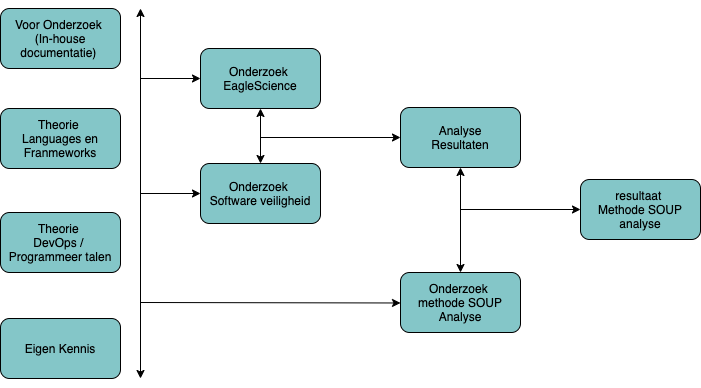
\includegraphics[width=10cm]{gfx/Onderzoekmodel}
    \caption{Onderzoeksmodel}
    \label{fig:OnderzoeksModel}
\end{figure}
In figuur\ref{fig:OnderzoeksModel} is te zien hoe de deelvragen in relatie staan met elkaar om samen tot een antwoord te komen op de vraag "Hoe kan EagleScience middels een dan al niet geautomtiseerde methode inzicht krijgen in potentiële kwetsbaarheden van gebruikte bibliotheken binnen zowel lopende als niet lopende projecten?". Om het overzicht en de scope te bewaren is er gekozen om iedere deelvraag apart te onderzoeken. In de komende secties is te lezen hoe deze aparte onderzoeken gedaan worden. In de hoofdstukken die volgen zullen de onderzoeken te lezen zijn en wat de conclussies zijn uit deze onderzoeken.

\section{Scope}\label{sec:Scope}
De wereld van software ontwikkeling is enorm en groeit met de dag Als ook de kennis en manieren om steeds veiliger software te maken. Om er voor te zorgen dat de onderzoeken relevant zijn voor de opdracht dient de volgende scope in acht te worden genomen:
\begin{itemize}
    \item Alleen de dev-stack van EagleScience is relevant. Oplossing die bestaan voor andere ontwikkeltalen en tooling wordt genoemd maar niet verder onderzocht.
    \item Sotware veiligheid is een breed veld en er wordt in dit onderzoek alleen gekeken naar het onderdeel wat gaat over het gebruik van externe bibliotheken. Om een relatie te bieden van dit onderdeel te opzichte van de rest worden andere onderdelen genoemd maar niet verder ingegaan.
    \item Er is veel beweging in het doen van analyses op source code. en er zijn inmiddels een aantal tools beschikbaar die deze analyses kunnen doen. Echter veel van deze tools zijn niet opensource en vragen een dergelijke aanpassing in de huidige manier van werken dat er voor gekozen is deze buiten beschouwing te laten. Er worden alleen tools meegenomen die "makkelijk" te integreren zijn in de huidige buildstraat.
\end{itemize}

\section{Het onderzoek}\label{sec:methodeonderzoek}
Zoals hierboven is aangegeven zullen er een drietal onderzoeken worden uitgevoerd die ieders een deel van de gestelde onderzoeksvraag zullen beantwoorden. De conclussie van de eeste twee onderzoeken is input voor het laatste onderzoek wat een zoektocht is naar een methode die in te passen is in de huidige buildstraat conform de opdracht van de oprdrachtgever.
\section{Ondezoeken}\label{sec:onderzoeken}
De vooronderzoeken hebben ieders een eigen onderwerp, doel, onderzoeksvraag en methode
\subsection{Onderzoek 1: Architectuur binnen EagleScience}\label{subsec:onderzoeksmethode-architectuur-binnen-eaglescience}
Het \textbf{doel} van dit onderzoek is om kennis te vergaren over de manier van uitrollen van software binnen EagleScience. Daarnaast moet het onderzoek inzicht geven in de gebruikte dev-stack( programeertalen, tooling en frameworks). De uitkomst is relevant omdat het een basis is waar de nieuwe oplossing onderdeel van wordt. De \textbf{Scope} van dit onderzoek beperkt zich dan ook alleen op de processen van die direct iets te maken hebben met het ontwikkelen en uitrollen van de software. Uit het doel en de scope komt de volgende ~\textbf{onderzoeksvraag}: "Welke methode en dev-stack wordt er gebruikt om binnen EagleScience software te ontwikkelen en uit te rollen?". De \textbf{methodes} die gebruikt worden zijn de interne documenten over de verschillende platformen en werkwijzen die beschikbaar zijn gesteld door het bedrijf zelf. De kennis uit deze documenten kan worden aangevuld door informatie dat uit bronnen van leveranciers afkomstig is. Daarnaast zullen er gesprekken plaats vinden met collega's. Deze input geeft het volgende onderzoeks model wat te zien is in figuur~\ref{fig:OnderzoeksModelEaglescience}
De \textbf{bronnen} die voornamelijk gebruikt worden zijn interne documenten waarin vermeld staat hoe een project verloopt en welke tooling er gebruikt wordt. Daarnaast zal er veel gebruik gemaakt worden van kennis van collega's en die ik zelf heb opgedaan dan al niet tijdens mijn opleiding.
\begin{figure}[htbp]
    \myfloatalign
    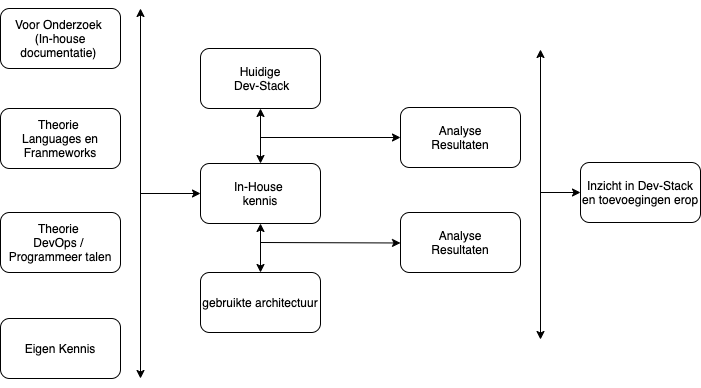
\includegraphics[width=10cm]{gfx/OnderzoeksmodelES}
    \caption{Onderzoeksmodel Eaglescience}
    \label{fig:OnderzoeksModelEaglescience}
\end{figure}


\newpage % quickfix om volgordelijkheid te veranderen voor figuren...


\subsection{Onderzoek 2: Literatuur studie veiligere software door SOUP analyse}\label{subsec:onderzoek-literatuur-studie-soup}
nieuwe vraag: "Wat is het effect van gebruik van externe bibliotheken bij het ontwikkelen van software, welke gevaren brengt dit met zich mee en wat kan er gedaan worden om deze gevaren te minimaliseren?"
Het \textbf{doel} van dit onderzoek is om inzicht te krijgen wat een SOUP-analyse is en hoe relevant het is om dit te doen. Daarnaast wordt er gekeken wat de SOUP-analyse toevoegd aan de veiligheid van de software die EagleScience levert. Met dit doel is de \textbf{scope} dat er alleen gekeken wordt naar soup-analyses en dat andere methoden die software veiliger maken wel aanbod komen als referentie. Maar niet verder worden uitgezocht.  De \textbf{onderzoeksvraag} luid: "Hoe kan SOUP op een effectieve manier worden geanalyseerd en hoe maakt dit software veiliger?". De gebruikte \textbf{methodes} zullen deskresearch zijn aangevuld met interviews. Interviews met collega's zullen inzicht brengen in methodes die al worden toegepast om software veiliger te maken. Daarnaast zijn een aantal conferenties die gehouden worden met software veiligheid als onderwerp. Deze conferenties staan nu door de huidige wereld situatie online en zijn vaak terug te kijken. Het onderzoeksmodel welke te zien is in figuur~\ref{fig:OnderzoeksModelNoodZaakSOUP} geeft een beeld hoe de methoden worden toegepast om tot een eindresultaat te komen. De \textbf{bronnen} die gebruikt zullen worden zullen online bronnen zijn aangevuld met vraaggesprekken met collega's en medewerkers van instanties die zich bezighouden met het veiliger maken van software. Daarnaast worden relevante presentaties van conferenties terug gekeken voor verdere informatie.
\begin{figure}[htbp]
    \myfloatalign
    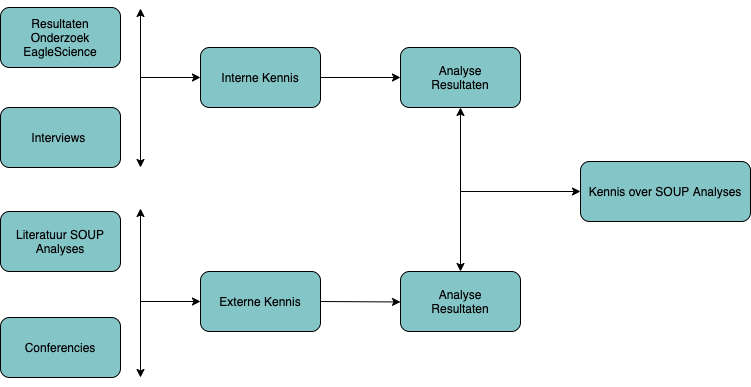
\includegraphics[width=10cm]{gfx/OnderzoeksmodelSOUP}
    \caption{Onderzoeks model gevaren van SOUP}
    \label{fig:OnderzoeksModelNoodZaakSOUP}
\end{figure}

%
%Dit onderzoek is vooral bedoeld om wegwijs te raken in de wereld het zoeken naar kwetsbaarheden binnen externe bibliotheken.
%Het gaat voornamelijk in op de betekenis van de verschillende begrippen en vervolgens hoe belangrijk het is om deze analyse uit te voeren.
%De uitkomst van dit onderzoek is een basis kennis die als entree voor de komende onderzoeken gebruikt kan worden.
%Het onderzoek heeft niet echt een hoofdvraag waardoor er een duidelijke scope moet worden gedefineerd.
%De volgende zaken moet duidelijk worden in dit onderzoek:
%\begin{itemize}
%  \item "Wat is SOUP?"
%  \item "Waarom kan het gebruik van SOUP gevaarlijk zijn?"
%  \item "Hoe worden deze gevaren/kwetsbaarheden gelogd?"
%  \item "Wat is een CVE en een CVSS?"
%\end{itemize}
%
%
%

\newpage % tijdelijk om te zorgen dat figuur op zelfde pagina als tekst komt
\subsection{Onderzoek 3: Implementatie van een SOUP-analyse}\label{subsec:onderzoek-naar-soup-analyse}
Het \textBF{doel} is om een tooling/bibliotheken te vinden die gebruikt kan worden om soup analyses te doen die binnen de huidige methode van uitrollen van eaglescience past. Daarnaast moet in kaart worden gebracht welke output deze methode genereert zodat het input geeft in de nieuwe oplossing. De \textbf{methode} die gebruikt wordt is deskresearch om te onderzoeken welke tooling er bestaat. Als er een selectie is gemaakt voor een tool dient deze in een kleine testopstelling getest te worden om vervolgens te kijken of we deze kunnen implementeren in de bestaande uitrolmethode. De \textbf{bronnen} die gebruikt zullen worden zijn informatie bronnen van leveranciers van dergelijke tooling. Daarnaast zullen de bevindingen middels een review worden geverifieerd op bruikbaarheid bij de opdrachgever. Het onderzoeksmodel voor dit onderzoek is te vinden in figuur~\ref{fig:OnderzoeksModelSOUPmethode}

\begin{figure}[htbp]
    \myfloatalign
    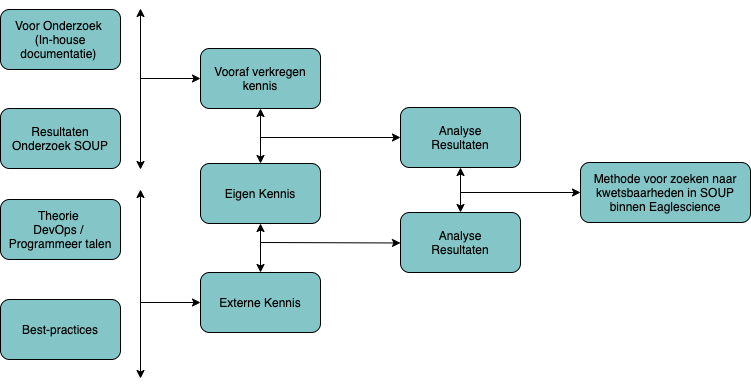
\includegraphics[width=10cm]{gfx/OnderzoeksModelSOUPMethode}
    \caption{Onderzoeksmodel SOUP-analyse module}
    \label{fig:OnderzoeksModelSOUPmethode}
\end{figure}
